\chapter{Activity Diagram} % Yutong

The activity diagrams shown in Figures~\ref{fig:act-div-usr} and \ref{fig:act-div-dev} describe the flow of actions when users and developers, respectively, access the application. The potential actions are based on the use cases described in Figure~\ref{fig:use-cases}.

Figure 4.1 is what the users can do with the system.
Through the system, the users can play the game as well as keep track of their progress. The users can choose to interact with a virtual child from their own perspective or interact with an adult from a child's perspective. 


Figure 4.2 is what the developers can do with the system.
Through the system, the developers can analyze collected user data and keep track of users' progress. With data analysis, the developers can detect "initial" stress, decide stress level, and measure current stress level for the users. By comparing the users' current stress level with the standard of their stress level, the developers can then personalize "training plan" for different users. 


\begin{figure}[!ht]
    \centering
    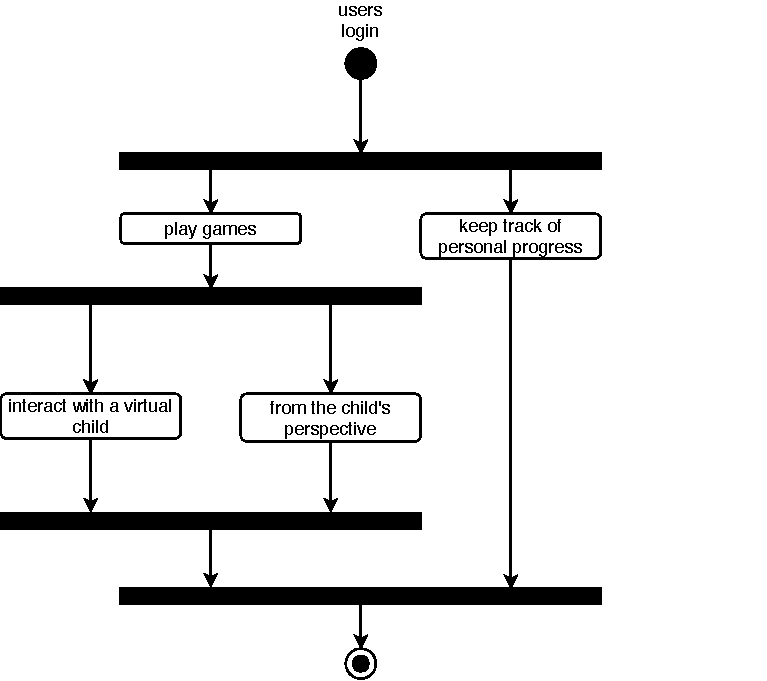
\includegraphics[width=0.75\linewidth]{activity-diagram-users}
    \caption{Users Activity Diagram}
    \label{fig:act-div-usr}
\end{figure}

\begin{figure}[!ht]
    \centering
    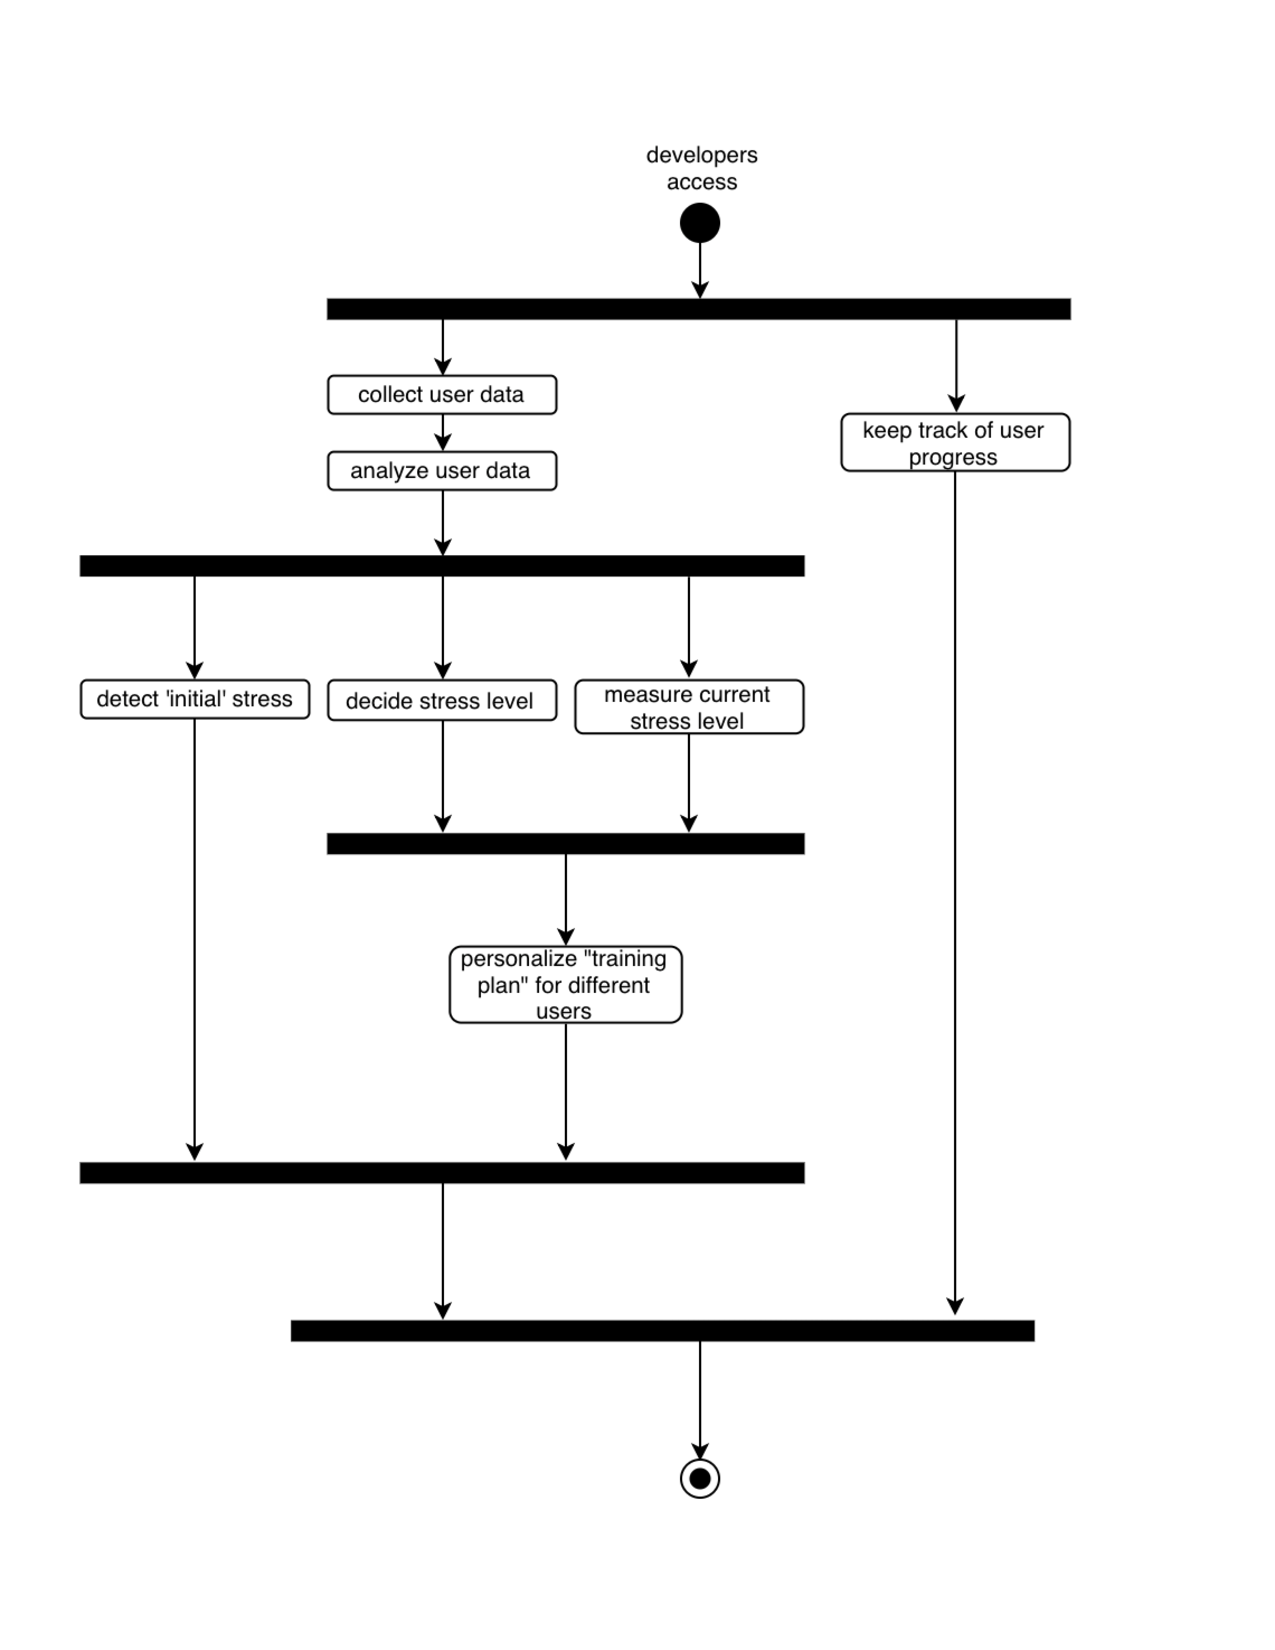
\includegraphics[width=\linewidth]{activity-diagram-developers}
    \caption{Developers Activity Diagram}
    \label{fig:act-div-dev}
\end{figure}